\subsection{Strong \& Weak Dominance}
\label{sec:dominance}

In our previous work of \ac{PBS} we presented the transaction dominance lattice (see Figure \ref{fig:category_lattice_2}) that establishes dominance of transactions that were categorized. While the prediction-based solution adds categorization to provide a solution against conflicting transactions, there is still the limitation that two transactions of the same categorization can be in conflict. In this situation, the prediction-based solution reverts to existing 2PL with no added benefit.

% \createCategorizationGraph{graph:cat_graph}{Categorization Graph}

\[\textrm{$HCHE > HCLE > LCLE$}\]
\[\textrm{$HCHE > LCHE > LCLE$} \]

\begin{figure}[h]
\captionsetup{justification=centering}
\centering % used for centering Figure

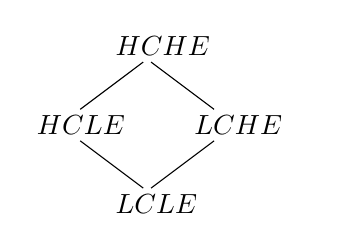
\begin{tikzpicture}
    % [list/.style={rectangle split, rectangle split parts=3,
    % draw, rectangle split horizontal}, >=stealth, start chain]
  \node[text width=1.5cm] at (4.4,5) {$HCHE$};
  \node[text width=1.5cm] at (3.4,4) {$HCLE$};
  \node[text width=1.5cm] at (5.4,4) {$LCHE$};
  \node[text width=1.5cm] at (4.4,3) {$LCLE$};
  \draw (4.0,4.8) -- (3.2,4.2);
  \draw (4.1,4.8) -- (4.9,4.2);
  \draw (4.0,3.2) -- (3.2,3.8);
  \draw (4.1,3.2) -- (4.9,3.8);
  
\end{tikzpicture}

\caption{Transaction Category Dominance} % title of the Figure
\label{fig:category_lattice_2} % label to refer figure in text

\end{figure}

By transitioning to a solution that contains a continuous spectrum of categorization, we can avoid the situation where two transactions of the same categorization cause a conflict. Tables \ref{tbl:read_lock_compatibility} \& \ref{tbl:write_lock_compatibility} show the existing rules for the four category solution. The existing operations would apply given the rules of dominance (see Definitions \ref{def:strong_dominance}, \ref{def:weak_dominance}, and \ref{def:not_comparable}) to execute and eliminate situations in which transactions of the same category would normally conflict.

Strong Dominance (see Definition \ref{def:strong_dominance}) is established when all four attributes of a reputation score of a transaction (commit ranking, efficiency ranking, user ranking, and system ranking) contain a value that is greater than all the values of the conflicting transactions reputation score. This the most preferred and easiest way to establish dominance between two conflicting transactions.

If Strong Dominance cannot be established then there is the ability to still obtain a "tie breaking" situation with Weak Dominance (see Definition \ref{def:weak_dominance}). Weak Dominance can be established by taking a sum of all four attributes of each transaction's reputation score and doing a numerical comparison of the overall score. If the score of the conflicting transaction is greater than or equal to the other transaction, then Weak Dominance is established preventing a stalemate.

If neither Strong or Weak Dominance can be established then we have reach a state of Not Comparable (see Definition \ref{def:not_comparable}). If the two conflicting transactions are deemed Not Comparable then the precedence of the two transactions will take priority and the conflicting transaction mus wait for the first transaction to complete.


% Figure \ref{image:vrm} displays a visual of the VRM solution where there are upper and lower bounds for reputation scores. This prevents transactional classes from being penalized or awarded to such an extent that they either cause starvation of other transactions or they suffer from starvation themselves. The plots along the vector represent the reputation scores of particular transactions. This figure gives a visual representation of the precedence of the transactions. Since the vector is not broken into four categories (see Figure \ref{graph:cat_graph} for a reference to our previous solution) there is a much granular and precise decision of which transaction takes precedence. With the VRM solution we no longer have to revert to 2PL for two transactions within the same category because we now have a numerical score that we can use for locking decisions.

% \begin{figure}
% \centering
% \includegraphics[scale=0.30]{images/VRM.png}
% \caption{Vector Reputation Management}
% \label{image:vrm}
% \end{figure}

% \begin{table}[h]
% \captionsetup{justification=centering}
% \centering
% \begin{tabular}{l|c|c|c|c|c|c|}

% \cline{2-5} & 
% \multicolumn{4}{c|}{\textbf{already granted lock}} \\

% \cline{2-5} \hline

% \multicolumn{1}{|l|}{\begin{tabular}[c]{@{}c@{}}\textbf{requested}\\\textbf{lock}\end{tabular}} &\textbf{$HCHE_{r}$}    & \textbf{$HCLE_{r}$}    & \textbf{$LCHE_{r}$}     & \textbf{$LCLE_{r}$}    \\ \hhline{=#====}
% \multicolumn{1}{|l||}{\textbf{$HCHE_{r}$}} &\textbf{+}    & \textbf{+}    & \textbf{+}     & \textbf{+}    \\ \hline
% \multicolumn{1}{|l||}{\textbf{$HCLE_{r}$}} &\textbf{+}    & \textbf{+}    & \textbf{+}     & \textbf{+}    \\ \hline
% \multicolumn{1}{|l||}{\textbf{$LCHE_{r}$}} &\textbf{+}    & \textbf{+}    & \textbf{+}     & \textbf{+}    \\ \hline
% \multicolumn{1}{|l||}{\textbf{$LCLE_{r}$}} &\textbf{+}    & \textbf{+}    & \textbf{+}     & \textbf{+}    \\ \hline
% \multicolumn{1}{|l||}{\textbf{$HCHE_{w}$}} &\textbf{-}    & $\delta$      & $\delta$       & $\delta$        \\ \hline
% \multicolumn{1}{|l||}{\textbf{$HCLE_{w}$}} &\textbf{-}    & \textbf{-}    & $\delta$       & $\delta$        \\ \hline
% \multicolumn{1}{|l||}{\textbf{$LCHE_{w}$}} &\textbf{-}    & \textbf{-}    & \textbf{-}     & $\delta$        \\ \hline
% \multicolumn{1}{|l||}{\textbf{$LCLE_{w}$}} &\textbf{-}    & \textbf{-}    & \textbf{-}     & \textbf{-}    \\ \hline           
% \end{tabular}

% \caption{Read-Lock Compatibility} % title of the Figure
% \label{tbl:read_lock_compatibility} % label to refer figure in text

% \end{table}


% \begin{table}[h]
% \captionsetup{justification=centering}
% \centering
% \begin{tabular}{l|c|c|c|c|c|c|}

% \cline{2-5} & 
% \multicolumn{4}{c|}{\textbf{already granted lock}} \\

% \cline{2-5} \hline

% \multicolumn{1}{|l|}{\begin{tabular}[c]{@{}c@{}}\textbf{requested}\\\textbf{lock}\end{tabular}} &\textbf{$HCHE_{w}$}    & \textbf{$HCLE_{w}$}    & \textbf{$LCHE_{w}$}     & \textbf{$LCLE_{w}$}    \\ \hhline{=#====}
% \multicolumn{1}{|l||}{\textbf{$HCHE_{r}$}} &\textbf{-}    & $\delta$    & $\delta$     & $\delta$    \\ \hline
% \multicolumn{1}{|l||}{\textbf{$HCLE_{r}$}} &\textbf{-}    & \textbf{-}    & $\delta$    & $\delta$    \\ \hline
% \multicolumn{1}{|l||}{\textbf{$LCHE_{r}$}} &\textbf{-}    & \textbf{-}    & \textbf{-}     & $\delta$    \\ \hline
% \multicolumn{1}{|l||}{\textbf{$LCLE_{r}$}} &\textbf{-}    & \textbf{-}    & \textbf{-}     & \textbf{-}    \\ \hline
% \multicolumn{1}{|l||}{\textbf{$HCHE_{w}$}} &\textbf{-}    & $\delta$      & $\delta$       & $\delta$        \\ \hline
% \multicolumn{1}{|l||}{\textbf{$HCLE_{w}$}} &\textbf{-}    & \textbf{-}    & $\delta$       & $\delta$        \\ \hline
% \multicolumn{1}{|l||}{\textbf{$LCHE_{w}$}} &\textbf{-}    & \textbf{-}    & \textbf{-}     & $\delta$        \\ \hline
% \multicolumn{1}{|l||}{\textbf{$LCLE_{w}$}} &\textbf{-}    & \textbf{-}    & \textbf{-}     & \textbf{-}    \\ \hline           
% \end{tabular}

% \caption{Write-Lock Compatibility} % title of the Figure
% \label{tbl:write_lock_compatibility} % label to refer figure in text

% \end{table}